\begin{figure}[t]
\centering
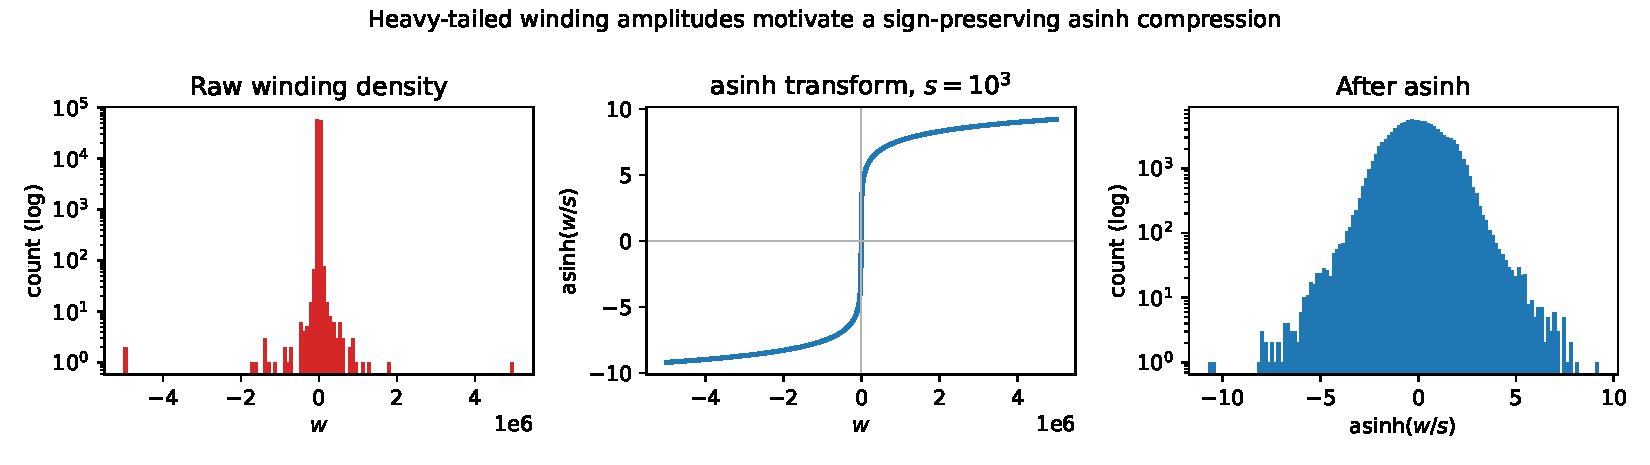
\includegraphics[width=\textwidth]{figures/fig_normalization.pdf}
\caption[Amplitude normalisation]{\textbf{Heavy-tailed amplitudes motivate the
asinh transform.} Left: the raw winding-density distribution (log count) is
sharply peaked with tails reaching $\sim\!10^{7}$. Centre: the sign-preserving
asinh transform of Eq.~\eqref{eq:asinh}, linear near zero and logarithmic in the
tails. Right: after the transform the distribution is well-behaved and roughly
symmetric, suitable for training.}
\label{fig:norm}
\end{figure}
